% ------------------------------------------------------------------------------
% Este fichero es parte de la plantilla LaTeX para la realización de Proyectos
% Final de Grado, protegido bajo los términos de la licencia GFDL.
% Para más información, la licencia completa viene incluida en el
% fichero fdl-1.3.tex

% Copyright (C) 2012 SPI-FM. Universidad de Cádiz
% ------------------------------------------------------------------------------
\begin{comment}
En esta sección se detalla la situación actual de la organización y las necesidades de la misma, que originan el desarrollo o mejora de un sistema informático. Luego se presentan los objetivos y el catálogo de requisitos del nuevo sistema. Finalmente se describen las diferentes alternativas tecnológicas y el análisis de la brecha entre los requisitos planteados y la solución base seleccionada, si aplica.
\end{comment}

\label{chapter:requisitos}

\section{\IfLanguageName{english}{Current Situation}{Situación actual}}
\begin{comment}
Esta sección debe contener información sobre la situación
actual de la organización para la que se va a desarrollar el sistema software.
\end{comment}
Como se ha explicado anteriormente en el capítulo \ref{chapter:introduccinon}, el presente proyecto nació con la necesidad de mejoras del \gls{framework} de búsqueda \gls{kf} aplicándose como modelo piloto al proyecto \gls{strada}.

\begin{comment}
\question{que situación actual de la organización y las necesidades de la misma, que originan el desarrollo o mejora de un sistema informático?? expuesto en la introducción \ref{section:alcance}}
\end{comment}

\subsection{\IfLanguageName{english}{Business Process}{Procesos de Negocio}}
\begin{comment}
Esta sección debe contener información sobre los modelos de procesos de negocio actuales, que suelen ser la base de los modelos de procesos de negocio a implantar.
\end{comment}

A continuación se detallan los procesos de negocio principales del proyecto \gls{kf} que actualmente están implantados.

\subsubsection{Importación de los datos}
En este proceso de negocio se produce la importación de los datos provenientes de un único repositorio de \gls{svn}. En el proceso implantado es necesario tanto permisos para poder obtener los datos del repositorio remoto como una copia local, previamente descargada. En la imagen \ref{image:negimport1} se representa el modelo proceso de este negocio en \gls{uml}.

\begin{figure}[H]
  \centering
    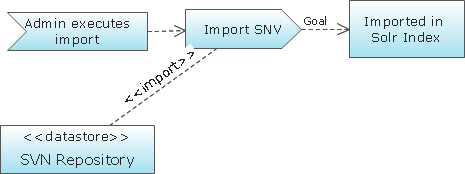
\includegraphics[width=0.8\textwidth]{NegocioOldImport.png} 
  \caption{Modelo de proceso de negocio, importación de los datos en \gls{kf}}
  \label{image:negimport1}
\end{figure}

\subsubsection{Búsqueda en el portal}
Este proceso de negocio se produce cuando el usuario filtra el conjunto de documentos usando para ello la interfaz web. Como resultado de la acción, el usuario obtiene una lista acorde con el filtro aplicado.  En la imagen \ref{image:negsearch1} se representa el modelo proceso de este negocio en \gls{uml}.

\begin{figure}[H]
  \centering
    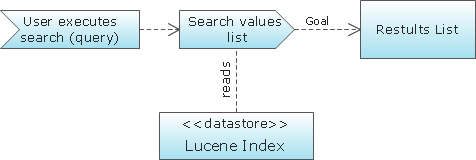
\includegraphics[width=0.8\textwidth]{NegocioOldSearch.png} 
  \caption{Modelo de proceso de negocio, búsqueda en el portal \gls{kf}}
  \label{image:negsearch1}
\end{figure}


\subsection{\IfLanguageName{english}{Technological Environment}{Entorno
Tecnológico}}
\begin{comment}
Esta sección debe contener información general sobre el entorno tecnológico en la organización del cliente antes del comienzo del desarrollo del sistema software, incluyendo hardware, redes, software, etc.
\end{comment}
\label{subsection:entornotech}

\sparagraph{Construcción}
La versión de la que se parte de \gls{kf} está implementada usando \Gls{jsdk} 6 Update 45 y \gls{maven} para la construcción del producto unificando todas sus partes, en la figura \ref{image:mavenkf} se puede observar un esquema de la organización de los archivos de configuración de \gls{maven} para esta versión del proyecto.\\

\begin{figure}[H]
  \centering
    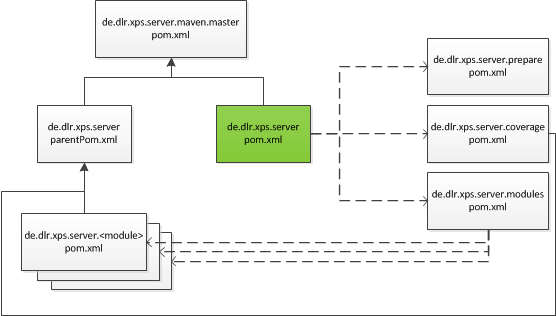
\includegraphics[width=0.8\textwidth]{DevDoc_PomStructure.png}
  \caption{Estructura simplificada de \gls{maven} en \gls{kf}}
  \label{image:mavenkf}
\end{figure}

Dado el portal donde se aloja la información de los institutos a los que está destinado \gls{kf} es \gls{liferay}, para esta versión del proyecto se implementó como contenedor un \gls{portlet} para \gls{liferay} 6.1 CE GA2 (6.1.1) sobre un servidor \gls{tomcat} 6.

\sparagraph{Importación}
A través de la lectura del repositorio remoto una copia local se extraen los dados de los documentos y se genera un índice de búsqueda en la fase de importación. Éste es índice es una instancia de \gls{lucene} en su version 3.0.2.\\

\sparagraph{Índice de búsqueda}
Partiendo de los datos del portal \gls{cs} (imagen \ref{image:csdata}) y del portal \gls{monitor} (imagen \ref{image:modata}) se crea durante la importación de los datos un índice de búsqueda con las propiedades expuestas en la imagen \ref{image:stradadata} para la instancia \gls{strada} del \gls{framework} \gls{kf} usada como referencia \cite{dublinstrada}.


\begin{figure}[H]
  \centering
    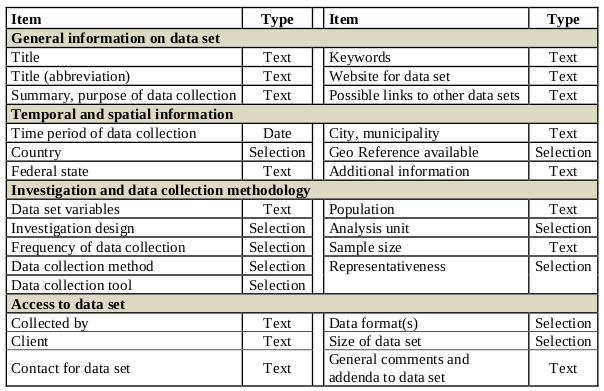
\includegraphics[width=0.8\textwidth]{cs_dublin.png} 
  \caption{\Glspl{metadato} de \gls{cs} \cite{dublinstrada}}
  \label{image:csdata}
\end{figure}

\begin{figure}[H]
  \centering
    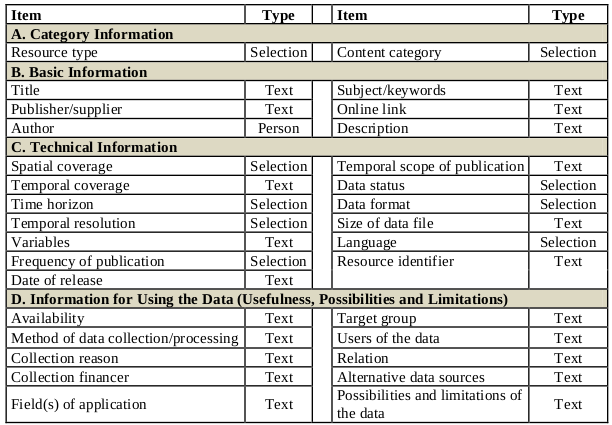
\includegraphics[width=0.8\textwidth]{monitor_dublin.png} 
  \caption{\Glspl{metadato} de \gls{monitor} \cite{dublinstrada}}
  \label{image:modata}
\end{figure}

\begin{figure}[H]
  \centering
    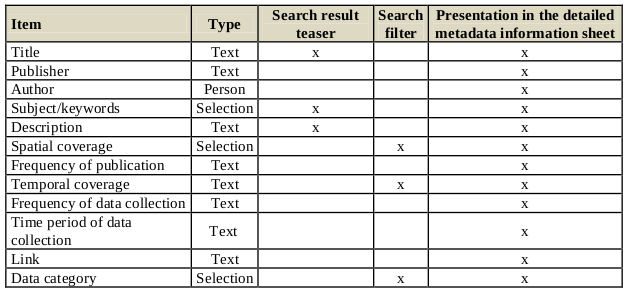
\includegraphics[width=0.8\textwidth]{strada_dublin.png} 
  \caption{\Glspl{metadato} de \gls{strada} \cite{dublinstrada}}
  \label{image:stradadata}
\end{figure}

\sparagraph{Interfaz de usuario}
Para la realización de la página web se utilizó el \gls{framework} de programación web  \gls{vaadin} 6. Únicamente usando sus componentes predefinidos se implementó la interfaz de usuario y su funcionalidad.\\

Junto con la configuración de un tema de \gls{liferay} por cada instancia del \gls{framework} (\gls{elib}, \gls{monitor} y \gls{strada}del se terminó de perfilar la apariencia y el comportamiento de la interfaz.

\sparagraph{Configuración}
Exceptuando la importación de los datos que se configura a nivel de parámetros en la ejecución, la configuración y adaptación del \gls{kf} para los distintos escenarios se realiza a nivel de código, es decir, que para cada instancia que se implemente hay que editar el \gls{framework} para adaptarlo a las necesidades específicas requeridas.


\subsection{\IfLanguageName{english}{Weakness and Strong Points}{Fortalezas y Debilidades}}
\begin{comment}
Esta sección debe contener información sobre los aspectos positivos y negativos del negocio actual de la organización para la que se va a desarrollar el sistema software.
\end{comment}
La implementación del \gls{framework} \gls{kf} presenta unos aspectos positivos y negativos que se pueden agrupar en los siguientes puntos:

\begin{itemize}
\sitem{Importación de los datos y el índice de búsqueda}
Como anteriormente se ha comentado, para la importación de los datos en el índice de \gls{lucene} es necesario contar con una copia local del repositorio \gls{svn} y acceso al repositorio remoto. Esto representa un gran inconveniente durante la fase de desarrollo ya que el repositorio remoto es no debería de tener que ser modificado con datos de prueba durante el desarrollo.\\

Al obtener los datos también remotamente, el proceso de importación de los datos es dependiente tener acceso a este repositorio. Esto conlleva que el tiempo necesario para finalizar esta tarea se incremente notablemente y que el desarrollador siempre tenga que tener acceso a la red. En el código \ref{code:importkf1} se muestra un ejemplo de ejecución para importar los datos usando la linea de comandos. Por otra parte, esta simpleza hace que la importación se pueda ejecutar desde la linea de comandos o, por ejemplo, desde algún sistema automático como \gls{cron}.

\begin{listing}
\begin{minted}[linenos,
               numbersep=5pt,
               frame=single,
               framesep=2mm]{bash}
               
java -Xmx512m -jar
de.dlr.xps.server.datafinder.indexer.fw-jar-with-dependencies.jar 
--idx-path D:\Projects\xps\index\fw-test-data
--svn-username user 
--svn-password ********
--svn-url https://svn.sistec.dlr.de/svn/xps/fw-test-data/ 
--svn-working-copy-path "D:\Repositories\fw-test-data\data\dat" 
--parse-content

	\end{minted}
	\caption{Ejemplo de importación de datos en \gls{kf}.}
	\label{code:importkf1}
\end{listing}


\sitem{Configuración de las nuevas instancias}
Cada instancia del \gls{framework} \gls{kf} tiene distintos datos. Para configurar estos datos es necesario reimplementar el proyecto ya que la tratamiento de los datos está incluido en el código fuente. Esto implica, a pesar de un proceso de refactorización aplicado sobre el \gls{software}, una duplicación de código para cada instancia del \gls{framework}. En la actualidad hay tres instancias en producción o desarrollo (\gls{monitor}, \gls{strada} y un último proyecto en fase de estudio \gls{elib}) lo que causa que exista una gran replicación de código dificultando considerablemente su desarrollo y mantenimiento.\\ 

A modo indicativo en la imagen \ref{image:eclipsekf} vemos la estructura del programa importado en \gls{eclipse}. Los módulos o paquetes acabados en ``fw'' corresponden al proyecto \gls{monitor}, los acabados en ``cs'' al \gls{strada} y ``ly'' al \gls{elib}.

\begin{figure}[h!]
  \centering
    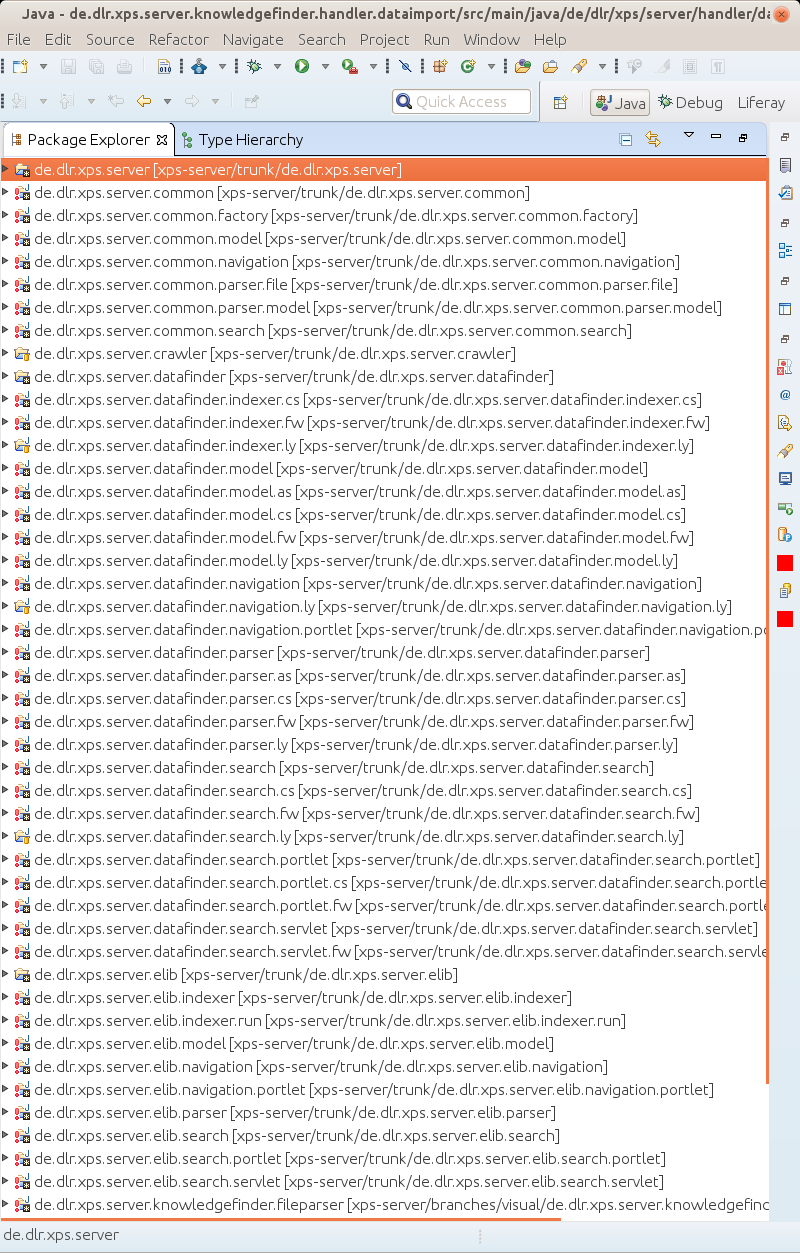
\includegraphics[width=0.7\textwidth]{eclipse.png}
  \caption{Las instancias del proyecto \gls{kf} en \gls{eclipse}}
  \label{image:eclipsekf}
\end{figure}

\sitem{La interfaz de usuario y la comunicación con el servidor}
Como se ha comentado en el apartado anterior, la interfaz de usuario está implementada usando una versión no actual de \gls{vaadin}, sin soporte técnico desde mayo de 2014. En el código del \gls{kf} es confuso, complejo y no se encuentra bien estructurado el sistema de tal forma que dentro del mismo proyecto no se puede diferenciar claramente entre los módulos, por ejemplo, de la interfaz de usuario y la importación de los datos.\\

Esta complejidad hace también que el mantenimiento y adaptación de la interfaz de usuario sea más tediosa y laboriosa.\\

En lo que respecta al tipo de tecnología, el \gls{framework} \gls{vaadin} necesita una constante comunicación con el servidor provocando que por cada interacción con el sistema el usuario tiene que esperar una respuesta del servidor.\\

El sistema de búsqueda de \gls{kf} está centrado y limitado al texto, tanto el sistema de búsqueda como la representación de los datos. A pesar de que los relación datos presentan una más compleja, estas relaciones no se muestran de forma directa. En la imagen \ref{image:monitor} se puede apreciar los distintos componentes de la interfaz para \gls{monitor}.

\begin{figure}[h!]
  \centering
    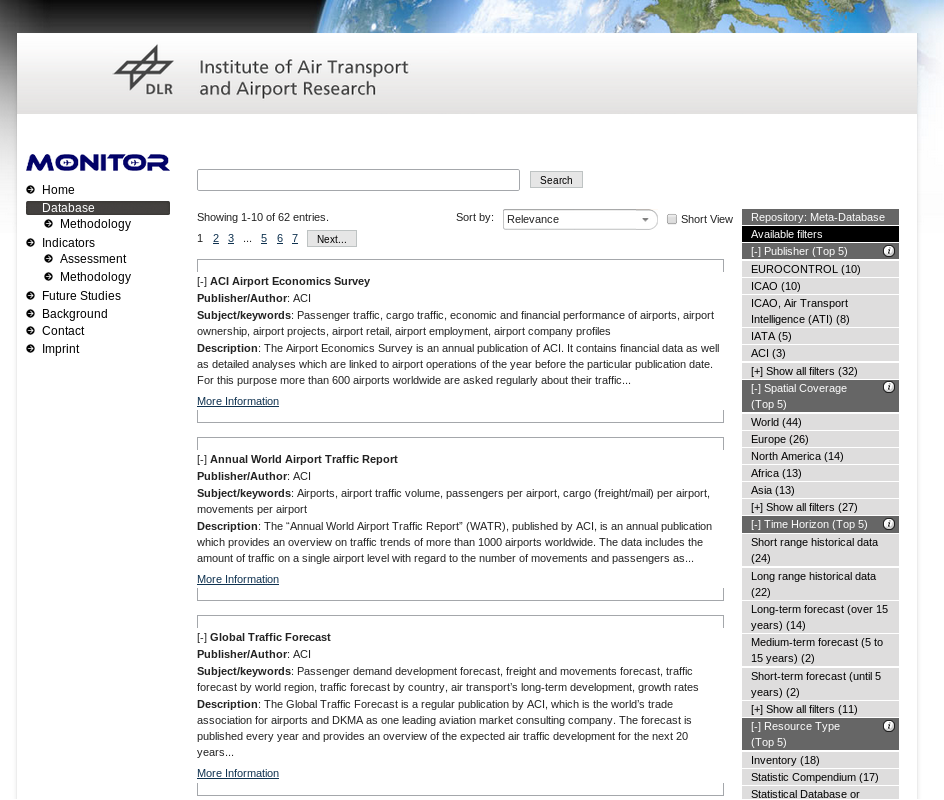
\includegraphics[width=0.8\textwidth]{monitor.png}
  \caption{Interfaz de usuario para \gls{monitor}}
  \label{image:monitor}
\end{figure}
\end{itemize}


% vaadin, lento pero en Java todo. nuevos componentes de UI muy complejo de crear si no existen en vaadin, combinar JS con JAVA usando GTW.


\section{\IfLanguageName{english}{Business Needs}{Necesidades de Negocio}}
%Esta sección debe contener información sobre los objetivos de negocio de clientes y usuarios, incluyendo los modelos de procesos de negocio a implantar.

A continuación se exponen los objetivos de negocio de clientes y usuarios, junto a los modelos de proceso de negocio, del proyecto \gls{kf2}
 
\subsection{\IfLanguageName{english}{Business Goals}{Objetivos de Negocio}}
Los objetivos de negocio de \gls{kf2} son:
\begin{itemize}
	\sitem{Simplificar adaptación del \gls{framework} para las distintas instancias}
    El nuevo \gls{kf2} tiene que ser un sistema que se adapte fácilmente a los distintos sistemas de conocimiento. Tanto el sistema de importación como la representación para el usuario debe ser fácilmente configurable y extensible.
    
    \sitem{Visualización gráfica del conocimiento}
	Para esta nueva versión del \gls{framework} se debe obtener una visualización gráfica del conocimiento que represente las relaciones y las estructuras complejas que existen los distintos \glspl{metadato}. A través de esta visualización el usuario deberá obtener una visión conjunta estas estructuras facilitando de esta forma la búsqueda de documentos. 
\end{itemize}
% \question{no es lo mismo que alcance de la sección de introducción \ref{chapter:introduccion}}
% Esta sección debe contener los objetivos de negocio que se esperan alcanzar cuando el sistema software a desarrollar esté en producción.

\subsection{\IfLanguageName{english}{Business Process}{Procesos de Negocio}}
% Esta sección, debe contener los modelos de procesos de negocio a implantar, que normalmente son los modelos de procesos de negocio actuales con ciertas mejoras.

En esta sección se exponen los procesos de negocio del \gls{framework} \gls{kf2}.

\subsubsection{Importación de los datos}
En este proceso de negocio se produce la importación de los datos provenientes de repositorios de \gls{svn} configurados. En la imagen \ref{image:negimport2} se representa el modelo proceso de este negocio en \gls{uml}.

\begin{figure}[H]
  \centering
    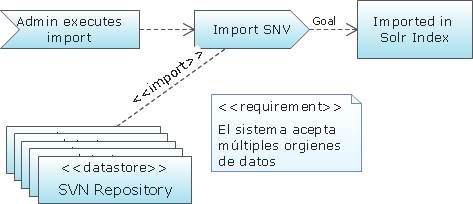
\includegraphics[width=0.8\textwidth]{NegocioNuevoImport.png} 
  \caption{Modelo de proceso de negocio, importación de los datos en \gls{kf2}}
  \label{image:negimport2}
\end{figure}

\subsubsection{Búsqueda en el portal}
Este proceso de negocio se produce cuando el usuario filtra el conjunto de documentos usando para ello la interfaz web. Como resultado de esta acción, el usuario obtiene una lista acorde con el filtro aplicado y una visualización de los documentos.  En la imagen \ref{image:negsearch2} se representa el modelo proceso de este negocio en \gls{uml}.

\begin{figure}[H]
  \centering
    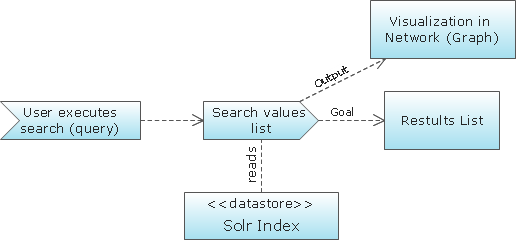
\includegraphics[width=0.8\textwidth]{NegocioNuevoSearch.png} 
  \caption{Modelo de proceso de negocio, búsqueda en el portal \gls{kf2}}
  \label{image:negsearch2}
\end{figure}

\section{Obtención de los Objetivos del Sistema}
Una vez extraídas las nuevas necesidades de negocio, era necesario refinarlos para obtener los objetivos reales del sistema. El punto más dificultoso fue la elección del elemento de visualización a diseñar. Para obtener más detalles sobre qué aspectos eran más importantes, se realizó un sondeo entre los institutos involucrados.\\

Las visualizaciones que más se acercaban a las necesidades concretas fueron:
\begin{itemize}
	\item \textbf{Chord Diagram} (imagen \ref{image:corddiagram})
    \begin{figure}[H]
      \centering
    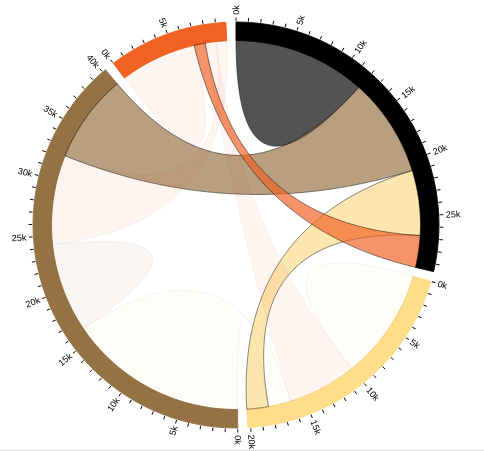
\includegraphics[height=0.35\textheight]{chord.png}
      \caption{Chord Diagram}
      \label{image:corddiagram}
    \end{figure}
    
   	\item \textbf{Bubble Chart} (imagen \ref{image:bubble})
     \begin{figure}[H]
      \centering
    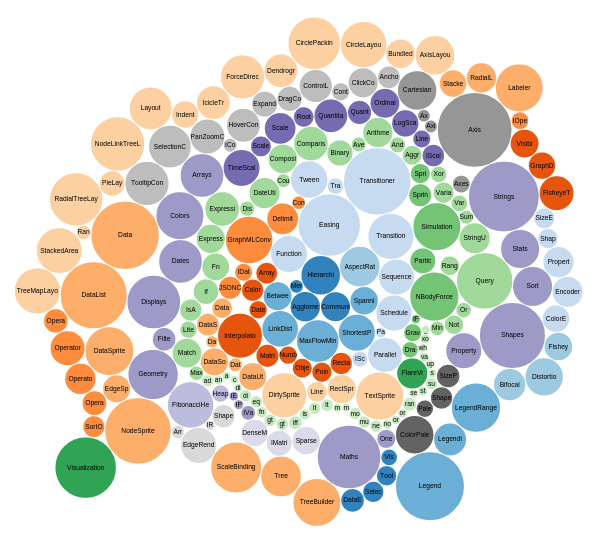
\includegraphics[height=0.35\textheight]{bubble.png}
      \caption{Bubble Chart}
      \label{image:bubble}
    \end{figure}

	\item \textbf{Circle Packing} (imagen \ref{image:packing})
     \begin{figure}[H]
      \centering
    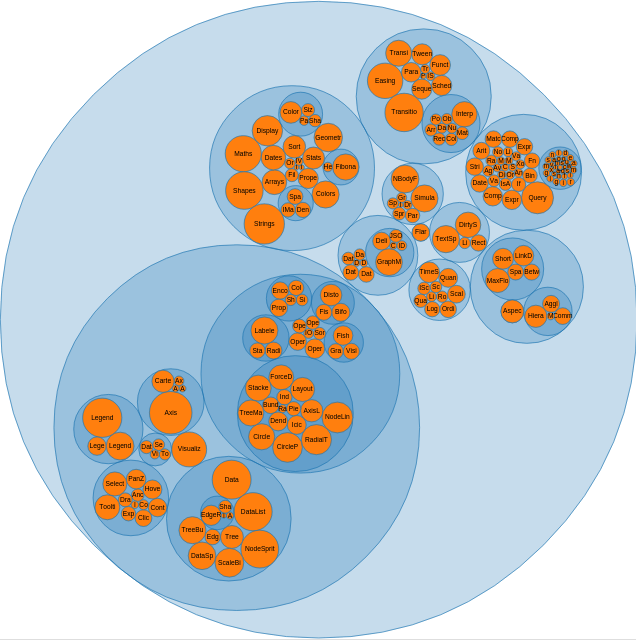
\includegraphics[height=0.35\textheight]{circle.png}
      \caption{Circle Packing}
      \label{image:packing}
    \end{figure}
	\item \textbf{Grafo - Force Layout} (imagen \ref{image:graphlayout})
     \begin{figure}[H]
      \centering
    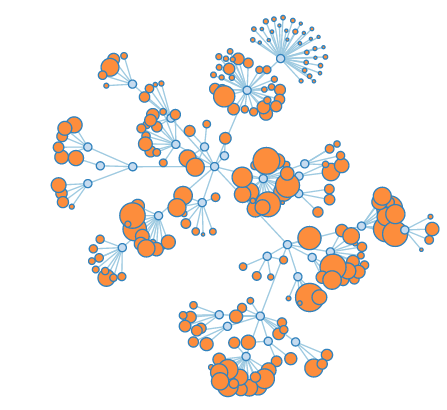
\includegraphics[height=0.35\textheight]{layout.png}
      \caption{Grafo - Force Layout}
      \label{image:graphlayout}
    \end{figure}
\end{itemize}

Tras varias conversaciones para saber qué propiedades eran las más interesantes de cada uno, se optó por el grafo de \glspl{metadato} como elemento central de la visualización para el proyecto ya que sus relaciones representan las estructuras complejas con más fidelidad y es más intuitivo para el usuario.

\section{\IfLanguageName{english}{System Goals}{Objetivos del Sistema}}
% \question{Objetivos del sistema? objetivos del negocio? que poner aqui??}Esta sección debe contener la especificación de los objetivos o requisitos generales del sistema.

% \question{Qué pasa con la obtención de requisitos, donde puedo incluir las entrevistas y ese proceso?}

\subsection{Importación y adaptación configurable}
El sistema de importación e indexación debe aceptar nuevos repositorios \gls{svn}. A su vez, el sistema encargado de la \gls{ui} debe ser igualmente configurable y extensible a través de ficheros de configuración para adaptarse las peculiaridades de cada portal.

\subsection{Representación de los \glspl{metadato} en un grafo}
Los \glspl{metadato} extraídos durante el proceso de indexación se deben mostrar en un grafo interactivo junto con sus relaciones. A través de este grafo, el usuario podrá definir sus criterios de búsquedas.


\section{\IfLanguageName{english}{System Requirements}{Catálogo de Requisitos}}
%Esta sección debe contener la descripción del conjunto de requisitos específicos del sistema a desarrollar para satisfacer las necesidades de negocio del cliente.
A continuación, en este apartado se describen los requisitos del proyecto \gls{kf2}.

\subsection{Requisitos de interfaces externas}

A continuación se describirán los requisitos de conexión con otros sistemas de software con los que el sistema va a interactuar para la importación de los \glspl{metadato} así como la \gls{ui}.

\subsubsection{Importación de los datos externos}
La importación de la información del portal se realizará partiendo de uno o varios repositorios de \gls{svn}. Estos repositorios podrán ser remotos, necesitando en su caso autenticación, o una copia de trabajo local. La información de los valores a importar se encontrará en las propiedades de \gls{svn} en formato \gls{json}.


\subsubsection{\Gls{ui}}
La \gls{ui} se usará por los usuarios para consultar con los datos indexados en el momento de la importación a través de un navegador web.\\

Los requisitos de la \gls{ui} del \gls{kf2} la podemos descomponer en los siguientes elementos; menú, grafo de exploración, selección actual, campo \gls{fulltext} y la lista de resultados.


\sparagraph{Menú}
Para una navegación clásica, el usuario dispondrá de un menú interactivo de navegación para gestionar los filtros que se desean aplicar a la búsqueda. Para este menú se requiere las siguientes características:

\begin{itemize}
\sitem{Multinivel}
El menú constará como máximo de dos subniveles de navegación y como mínimo uno.

\sitem{\Gls{scroll} en las opciones de menú}
Para las listar largas de opciones en el menú, éste debe de disponer de un \gls{scroll}.

\sitem{Contador de documentos por filtro en el menú}
En menú se dispondrán de un contador por cada filtro aplicable con el número de documentos que actualmente contienen el correspondiente filtro. 

\sitem{(Re)ordenación del menú}
Las opciones del menú obtenidas deben mantener el siguiente orden; primero las opciones seleccionadas y luego el resto de opciones ordenadas por el número que indique su contador de documentos correspondiente. 

\sitem{Grupos en acordeón}
La lista de elementos de un submenú deberán mostrarse dentro de un sistema de acordeón.
\end{itemize}

\subsubsection{Grafo de exploración}
Los \glspl{metadato} del conjunto de elementos importados deberán representarse en un grafo interactivo que muestre las relaciones entre ellos y la relevancia de éstos dentro del conocimiento en su totalidad.

\subsubsection{Selección actual}
En la interfaz de usuario se deben mostrar en una lista con los filtros actualmente han sido activados.

\subsubsection{Campo \gls{fulltext}}
La \glslink{ui}{interfaz} hará posible que el usuario pueda introducir texto libremente para que sea usado en el sistema de búsqueda.

\subsubsection{Lista de resultados}
Los documentos resultado de la búsqueda deberán de ser mostrados en una lista. En esta lista se deben poder diferenciar claramente los distintos elementos que la componen. También deberá cumplir las siguientes propiedades: 

\begin{itemize}
\sitem{Lista de resultados en forma de acordeón}
La lista de resultados debe mostrar el título de cada uno de los documentos y la posibilidad de una pequeña visualización de resumen de algunos campos seleccionados usándose un sistema de acordeón.

\sitem{\Gls{paginacion} en los resultados}
Para un gran número de resultados, la lista debe ser mostrada usando una \gls{paginacion}.

\sitem{Ordenación en los resultados}
La lista de resultados deberá ser mostrada en un orden seleccionable por el usuario.

\sitem{Detalles de los documentos}
En sistema debe permitir seleccionar un documento de la lista de resultados y mostrar todos sus campos disponibles en una ventana emergente.

\sitem{Contador de elementos en lista}
Como parte de la interfaz, el usuario dispondrá de manera clara de un contador con el número total de documentos para estado actual de la búsqueda. 
\end{itemize}


\subsection{\IfLanguageName{english}{Functional Requirements}{Requisitos funcionales}}
\label{subsection:funcionales}
%Descripción completa de la funcionalidad que ofrece el sistema.

\sparagraph{Pliegue y despliegue de la lista de resultados}
La interfaz de usuario debe permitir el pliegue y despliegue de cada elemento de la lista de resultados o todos con una simple acción.

\sparagraph{Pliegue y despliegue del menú}
La interfaz de usuario debe permitir el pliegue y despliegue de los elementos de menú con subgrupos. El usuario podrá desplegar o contraer los subelementos por cada grupo del menú.

% funcional
\sparagraph{Aplicar filtro de \gls{metadato}}
Cuando el usuario pulse sobre un \gls{metadato} (en grafo de exploración o en el menú) se debe filtrar los resultados acorde con el \gls{metadato} seleccionado. Si pulsa una arista que comunica dos \glspl{metadato}, se aplicara el filtro de ambos.

% funcional
\sparagraph{Desactivar filtro de \gls{metadato}}
Cuando el usuario pulse sobre un \gls{metadato} en el menú que ya esté aplicado o sobre la lista de la actual selección, éste se desactivará. 

% funcional
\sparagraph{Texto informativo de \gls{metadato}}
Cuando el usuario se encuentre sobre un \gls{metadato} (en gráfica de visualización o en el menú) se debe mostrar un texto con información adicional sobre éste.

\sparagraph{Resaltado de \gls{metadato}}
Cuando el usuario se encuentre sobre un \gls{metadato} (en gráfica de visualización o en el menú) se deben resaltar los elementos relacionados en el grafo, el correspondiente en el menú y los documentos que contienen ese \gls{metadato}.

\sparagraph{Resaltado de los \glspl{metadato} de documentos}
Cuando el usuario se sitúe sobre un documento de la lista de resultados se deben resaltar los \glspl{metadato} y las relaciones entre ellos en el grafo y en el menú.

% funcional?
\sparagraph{Búsqueda en el \gls{fulltext}}
El usuario a través del campo de búsqueda \gls{fulltext} podrá realizar búsquedas aproximadas, combinadas con operadores disyuntivos o conjuntivos, búsqueda exacta de texto y expresiones regulares simples (!, ?, *, \dots).\\

% funcional?
\sparagraph{Detalles de los documentos}
En sistema debe permitir seleccionar un documento de la lista de resultados y mostrar todos sus campos disponibles, dependiendo de los roles del usuario, en una ventana emergente.  

% funcional
\sparagraph{Interacción del menú con el gráfico visual}
Desde el menú, el usuario podrá activar o desactivar los grupos de \glspl{metadato} se mostrarán en el gráfico.

\subsection{\IfLanguageName{english}{Not-functional Requirements}{Requisitos no funcionales}}
%Descripción de otros requisitos (relacionados con la calidad del software) que el sistema deberá satisfacer: portabilidad, seguridad, estándares de obligado cumplimiento, accesibilidad, usabilidad, etc.

%%%%%%%%%%%%%%%%%%%%
% no funcional
\sparagraph{Adaptación de los campos sistema de importación }
El sistema de importación de los datos debe ser fácilmente configurable para añadir o suprimir campos en el índice de búsqueda. 

\sparagraph{Adaptación del sistema de importación}
La incorporación de nuevos tipos de fuentes de datos (por ejemplo desde ficheros \gls{xml}) tiene que ser relativamente simple.

\sparagraph{Adaptable a los roles del usuario}
El sistema debe permitir la configuración y combinación de roles para personalizar el resultado de las consultas y los campos a mostrar.

% no funcional
\sparagraph{Compartición del estado del portal usando \gls{url}}
Partiendo del supuesto de que tienen los mismos permisos, los usuarios podrán compartir el estado de la búsqueda y de la visualización a través de la dirección \gls{url} generada.

% no funcional
\sparagraph{Comportamiento dinámico del elemento visual}
El elemento visual debe comportarse de forma dinámica, es decir, que por cada cambio que deba producirse en él no se deba redibujar todo el gráfico, sólo las partes implicadas.

\sparagraph{Interacción de los componentes}
Los componentes de la \gls{ui} deben interaccionar entre ellos en la medida de lo posible tal que el usuario no perciba un descenso del rendimiento de la aplicación.

% no funcional
\sparagraph{Tiempo de respuesta de la interfaz}
Tanto la visualización como la búsqueda tendrá tiempo de respuestas aceptables a las peticiones de un usuario con un sistema y conexión estándar. El usuario debe poder interaccionar con el sistema sin percibir la comunicación con el servidor.

% no funcinal
\sparagraph{Ampliable con futuros elementos gráficos}
En un futuro debe ser posible la fácil incorporación de nuevos elementos gráficos a la \gls{ui}. La inclusión de mapas y lineas de tiempo que interactúen con el resto de componentes debe ser simple y eficiente.

% no funcional
\sparagraph{Grafo debe ser fácilmente configurable}
Aspectos como la complejidad o el estilo del gráfico interactivo deben ser fácilmente configurable.

\sparagraph{Lista de resultados debe ser fácilmente configurable}
Aspectos como la paginación o las opciones de ordenación deben 
ser fácilmente configurables.

% no funcional
\sparagraph{El menú debe ser fácilmente configurable}
El menú con las opciones de filtrado debe ser configurable hasta dos niveles (orden, estilos, textos, subelementos, \gls{scroll}, desplegado, \dots).

\sparagraph{Actualización automática del menú}
En su último nivel, las opciones son obtenidas de forma automática en el momento de la primera carga de la página.

% no funcional
\sparagraph{El estado inicial del gráfico fácilmente configurable}
El gráfico de visualización por defecto mostrado en la visita inicial de la aplicación debe ser configurable con relativa simpleza.

%  no funcional
\sparagraph{Carga en paralelo de los componentes}
Los componentes que forman el \gls{ui} deben de generarse y actualizarse en paralelo dentro de las posibilidades de las tecnologías de visualización y del navegador que el usuario esté usando.

\sparagraph{Estilos configurables}
Los estilos de los componentes que forman la \gls{ui} deben de ser fácilmente configurables conjuntamente.

\subsection{\IfLanguageName{english}{Engine Rules}{Reglas de negocio}}
% En el desarrollo del sistema, hay que tener en cuenta las denominadas reglas de negocio, es decir, el conjunto de restricciones, normas o políticas de la organización que deben ser respetadas por el sistema, las cuales suelen ser cambiantes.
\sparagraph{\Gls{java}, el lenguaje de programación}
Dado el carácter piloto de \gls{kf2}, el proyecto debe ser desarrollado en la medida de lo posible en un lenguaje dominado por el personal del \gls{scvss}. En este caso \gls{java} debe de ser usado como lenguaje de programación para el sistema de indexación
 
\subsection{\IfLanguageName{english}{Information Requirements}{Requisitos de información}}
% En esta sección se describen los requisitos de gestión de información (datos) que el sistema debe gestionar.



El sistema de información de \gls{kf2} está basado en un índice de búsqueda \gls{nosql}. Se mantendrá el mismo esquema expuesto en la imagen \ref{image:stradadata} exceptuando los campos que representan intervalos de tiempo, por ejemplo ``Temporal Coverage''.  Estos campos del índice proporcionarán la fecha máxima y mínima para los valores posibles dados para simplificar posibles consultas usando fechas. En la tabla \ref{table:transformtab} se representa algunas transformaciones posibles.

\begin{center}
	\begin {table}[H]
	\centering
      \begin{tabular}{| c | c | c|}
      \hline
      \textbf{Valor} & \textbf{Fecha mín.} & \textbf{Fecha máx.}\\ \hline
      2003 - 2010 & 2003-01-01 & 2010-12-31 \\ \hline
          - 2010 			& NULL				& 2010-12-31   	\\ \hline
      2003 - 			& 2003-01-01 				& NULL  	\\ \hline
      2003-03 - 2010-11 			& 2003-03-01 				& 2010-11-31   	\\ \hline
      2003-03-10 - 2010-10-31 			& 2003-03-10 				& 2010-10-31   	\\ \hline
      \end{tabular}
    \caption{Tabla resumen de las transformaciones para los rangos de fechas}
    \label{table:transformtab}
  \end{table}
\end{center}

\subsection{Restricciones técnicas del sistema}

\sparagraph{\Gls{portlet} de \gls{liferay}}
La página web usada como interfaz de usuario debe ser un \gls{portlet} compatible con una versión actual de \gls{liferay}.

\sparagraph{Compatibilidad con \gls{html5}}
La aplicación debe ser compatible con \gls{html5} es decir con la amplia mayoría de los navegadores actuales. Por supuesto, el uso de la tecnología \gls{flash} no está permitido.



\section{Alternativas de Solución} 

%En esta sección, se debe ofrecer un estudio del arte de las diferentes alternativas tecnológicas que permitan satisfacer los requerimientos del sistema, para luego seleccionar (si procede) la herramienta o conjunto de herramientas que utilizaremos como base para el software a desarrollar.
\begin{comment}

Frontend: Vaadin, GTK, buscar otros, creando un nuevo elemento, muy complejo crear adaptar el comportamiento de los existentes
Backend: adaptar el anterior sistema de importación mejorar rendimiento de las consultas...

usando MVN Excpliarlo 
Frontend nuevo componente JS, con los frameworks ...Cytoscape, sigma.js cargar grafo desde Neo4j o RDF crear imagen Canvas, 
Backend o importancion, adaptar el anterior y crear un servicio web
rediseñarlo usando solr para mejorar la importacion 

Seguridad
control de acceso de los usuarios
MoltMT de solr security
Crear un servico web con filtro de usuarios

estilos:
CSS directamente o SASS

otras cosas:
crossfilter timeline zoom, futuras mejoras...
\end{comment}

A continación se expone el estudio de la solución propuesta para el \gls{framework} \gls{kf2}.

\subsection{Elección de la tecnología de visualización}
Para la visualización del grafo descrito anteriormente, es necesario usar tecnología \gls{js}. Entre las posibles soluciones destacan:

\subsubsection{\gls{sigma}}
Sigma es una biblioteca \gls{opensource} de \gls{js} pura dedicada exclusivamente al dibujo de grafos interactivos (dinámicos y estáticos)  en aplicaciones web. \\

Con una configuración por defecto, esta biblioteca permite la representación ajustado al contenedor del grafo en \gls{webgl} o, si el navegador web lo permite, en \gls{canvas}.\\

Gracias a su \gls{api} pública y adaptando la configuración, se puede conseguir fácilmente 
una personalización de cómo dibujar y de cómo interactúa el grafo. También permite que el desarrollador incluya su propia funcionalidad para la representación de los nodos y conexiones.\\

Entre las propiedades a destacar es su rendimiento para representar gráficos con un altísimo número de nodos, en la imagen \ref{image:sigma2} se puede observar la exploración de un gran grafo de una red social usando este \gls{software}. Por otra parte, en la imagen  \ref{image:sigma} se representa una captura de pantalla de un ejemplo más simple de \gls{sigma}.

\begin{figure}[h!]
  \centering
    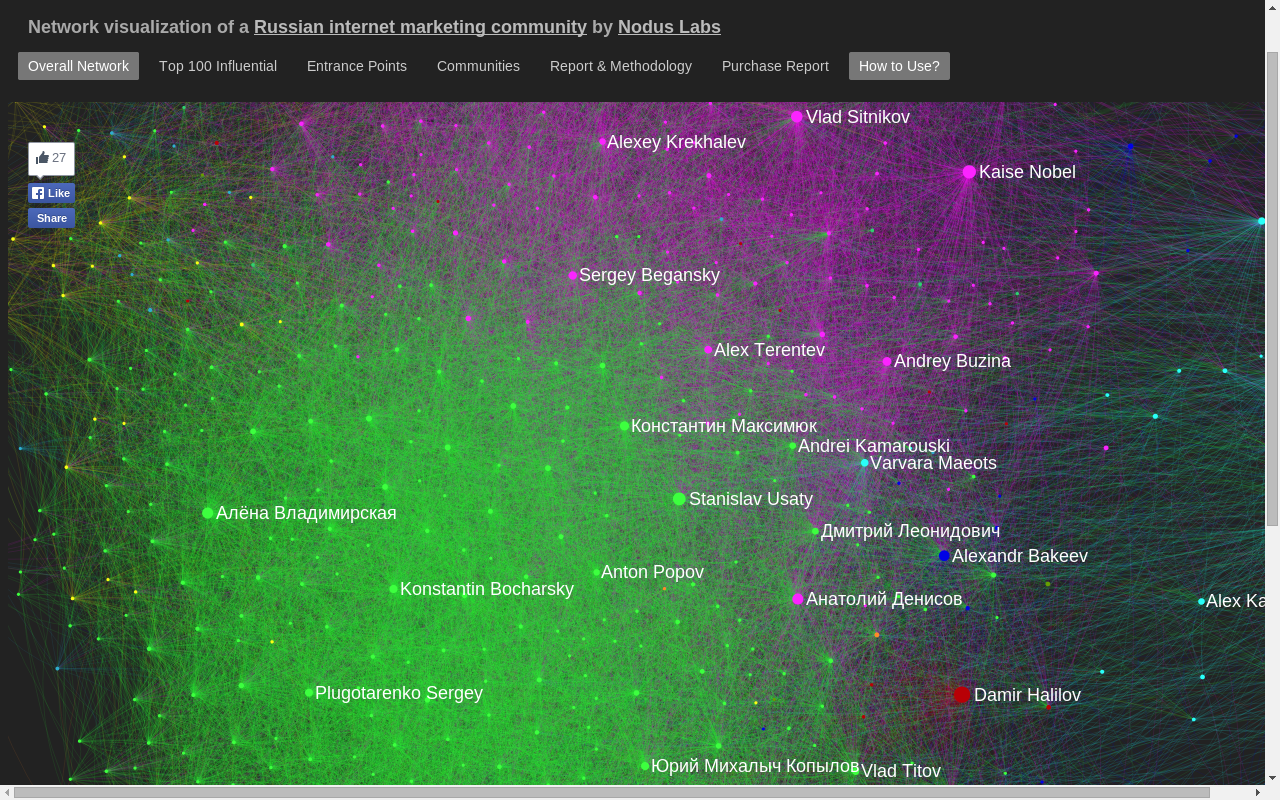
\includegraphics[width=0.8\textwidth]{sigma2.png}
  \caption{Exploración de una red social de marketing \gls{sigma} \cite{sigmaNodus}}
  \label{image:sigma2}
\end{figure}

\begin{figure}[h!]
  \centering
    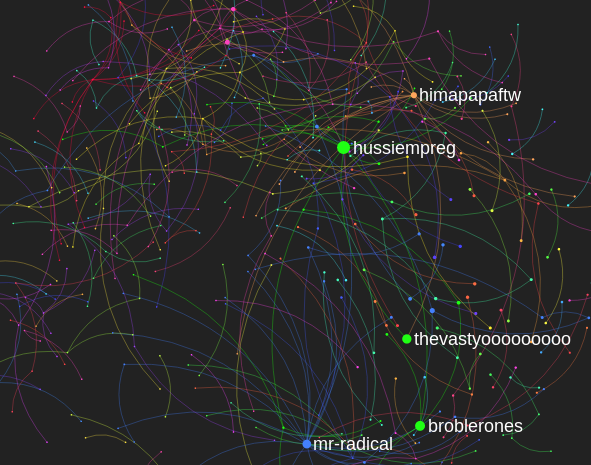
\includegraphics[width=0.7\textwidth]{sigmaTumblr.png}
  \caption{Exploración de la red de blogs Tumblr con  \gls{sigma} \cite{sigmaNodus}}
  \label{image:sigma}
\end{figure}

\subsubsection{\gls{cyto}}
\Gls{cyto} es una biblioteca \gls{opensource} escrita en \gls{js} para teoría de grafos, su visualización y análisis.\\

Permite la manipulación y representación de grafos interactivos facilitando al usuario crear sus propios eventos y personalizar la interacción con los grafos. Se integra con facilidad en las aplicaciones web y es compatible con los actuales navegadores.\\

En su biblioteca de funciones hay implementadas un conjunto de herramientas enfocadas a la teoría de grafos.\\

En la imagen \ref{image:cyto} podemos observar algunos ejemplos gráficos extraídos de su repositorio \cite{cyto}.

\begin{figure}[h!]
  \centering
    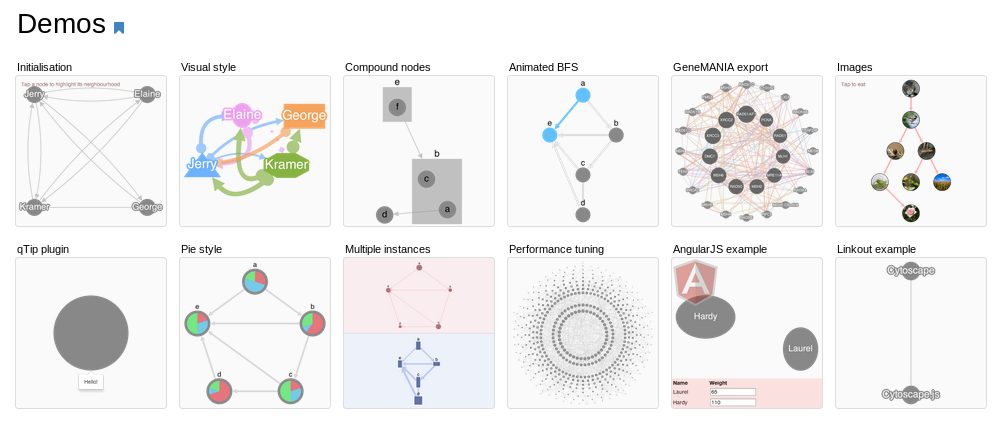
\includegraphics[width=0.9\textwidth]{cytoscape.png}
  \caption{Ejemplos visuales uso de \gls{cyto} \cite{cyto}}
  \label{image:cyto}
\end{figure}


\subsubsection{\gls{d3}}
\Gls{d3} es una biblioteca \gls{opensource} de \gls{js} para la manipulación de documentos basados en datos. Apoyándose en \gls{html5}, \gls{svg} y \gls{css} ayuda a mostrar a través de elementos visuales y manipular los datos de forma dinámica en aplicaciones web.\\

Una de sus bases es mantener los estándares facilitando  de esta forma que el \gls{software} desarrollado con él  sea compatible con los navegadores actuales.\\

La funcionalidad de \gls{d3} se basa en la conexión de la información con el \gls{dom} y la aplicación de transformaciones sobre el documento basado en unos en datos proporcionados. En el código \ref{code:d3data} podemos ver cómo de sencillo y simple se relacionan los datos con los componentes del \gls{dom}. En la imagen \ref{image:d3dataimage} el resultado interno de esta vinculación.\\


\begin{listing}
\begin{minted}[linenos,
               numbersep=5pt,
               frame=single,
               framesep=2mm]{javascript}
               
>>>> my_data = [20, 7, 32]
[20, 7, 32]
>>> d3.selectAll('.box').data(my_data).text( function(d) { return d } )
[[div.box, div.box, div.box]]

	\end{minted}
	\caption{Ejemplo de vinculación de datos con el \gls{dom} usando \gls{d3} \cite{D3exp2012}}
	\label{code:d3data}
\end{listing}

\begin{figure}[h!]
  \centering
    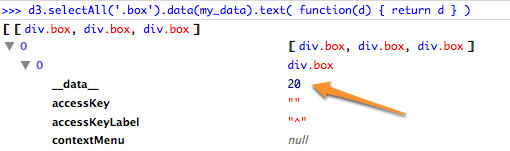
\includegraphics[width=0.7\textwidth]{domD3.png}
  \caption{Exploración del \gls{dom} después de la vinculación de datos \cite{D3exp2012}}
  \label{image:d3dataimage}
\end{figure}



Esta librería soluciona de forma eficiente la manipulación de documentos basados en datos y gracias a ello, permite que comportamientos dinámicos y de animación en los elementos visuales.\\

Todo esto junto con la claridad y calidad del código y la documentación de \gls{d3} facilita enormemente creación y reutilización de componentes visuales. Dentro de la biblioteca se encuentran ya definidos y extensamente documentados numerosos \glspl{plugin} visuales que ayudan para desarrollar nuestros propios elementos, adaptándose fácilmente a las necesidades de cada situación.\\

Uno de los puntos más fuertes de esta librería es su interacción entre los componentes y la facilidad de adaptación para usarse con otros sistemas. Por ejemplo, hacer funcionar \gls{d3} con la biblioteca para el uso de mapas \gls{leaflet} (imagen \ref{image:leaflet}) o con las gráficas de \gls{crossfilter} (imagen \ref{image:crossfilter}) es relativamente trivial.\\


\begin{figure}[h!]
  \centering
    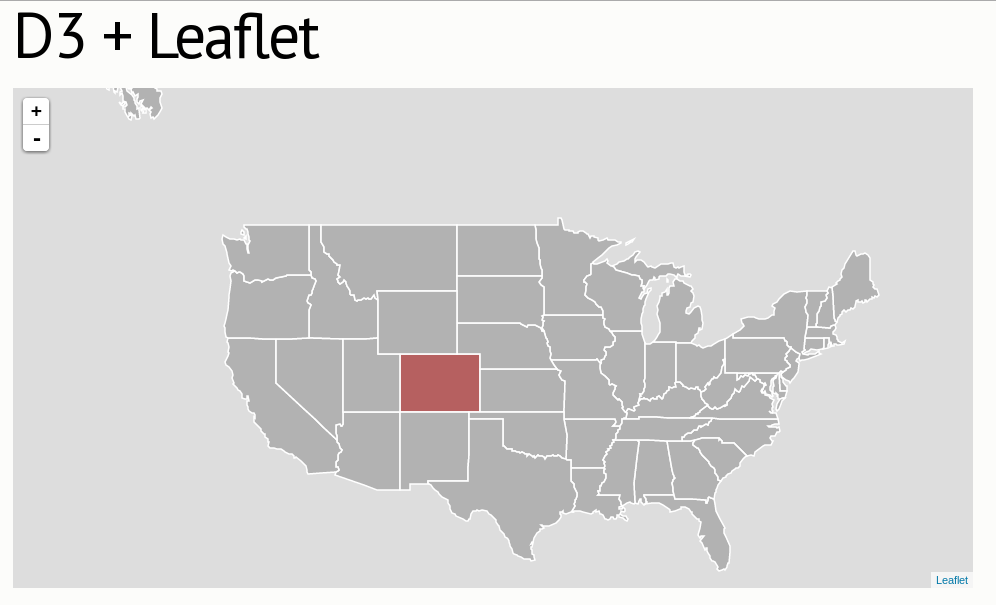
\includegraphics[width=0.8\textwidth]{leaflet.png}
  \caption{Ejemplo de integración de \gls{leaflet} con \gls{d3} usando mapas de GeoJSON \cite{d3leaflet}}
  \label{image:leaflet}
\end{figure}


\begin{figure}[h!]
  \centering
    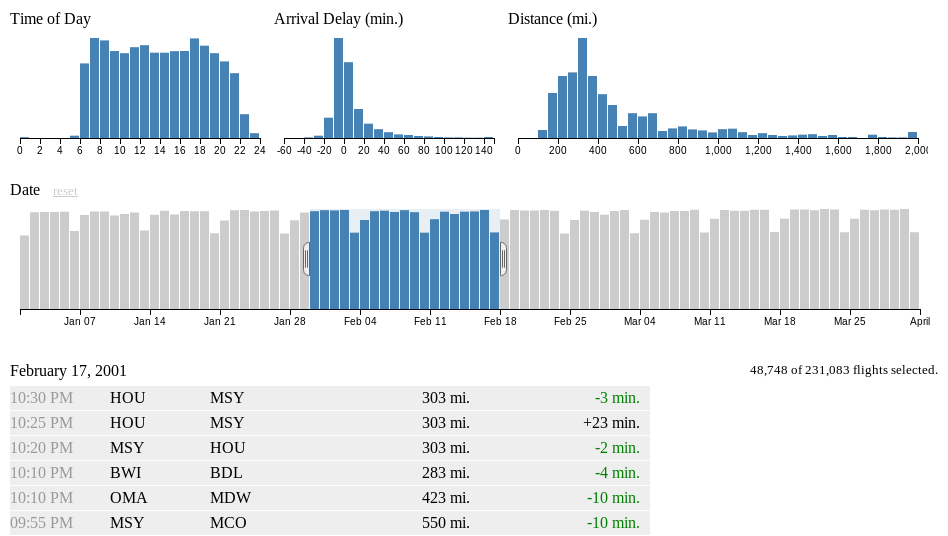
\includegraphics[width=0.8\textwidth]{crossfilter.png}
  \caption{Ejemplo de funcionamiento de \gls{crossfilter} \cite{crossfilter}}
  \label{image:crossfilter}
\end{figure}


Por otra parte, el gran número de ejemplos públicos desarrollado por terceros publicados bajo un mismo patrón bajo la dirección \url{http://bl.ocks.org/} hace que éstos puedan visualizarse directamente en la web y junto respaldado por una muy activa comunidad hacen que la labor del desarrollador sea productiva y eficaz. En la figura \ref{image:D3force} podemos observar uno de estos ejemplos aplicado a grafos.

\begin{figure}[h!]
  \centering
    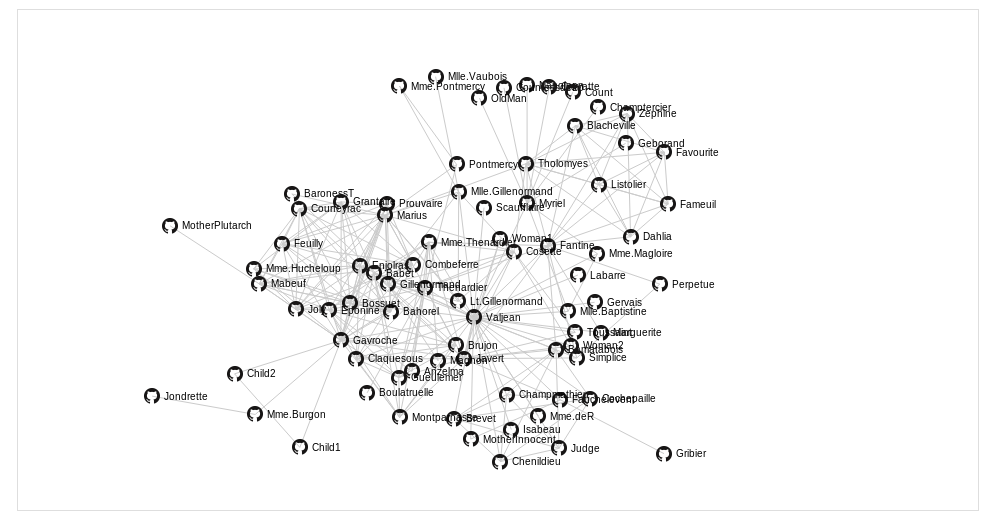
\includegraphics[width=0.8\textwidth]{D3force.png}
  \caption{Ejemplo de grafo en \gls{d3} publicado en \url{http://bl.ocks.org/mbostock/950642}}
  \label{image:D3force}
\end{figure}

\Gls{d3} trabaja sobre \gls{svg} por defecto para sus librerías gráficas. Esto tiene el inconveniente de que elementos visuales muy complejos tiene un bajo rendimiento.

\subsection{Elección del índice de búsqueda}
Para el proyecto \gls{kf} utilizó un índice de búsqueda \gls{lucene} en su versión 3.0.2. Dadas las restricciones provenientes de \gls{scvss} el índice de búsqueda del proyecto \gls{kf2} deberá basarse en éste.\\

Por este motivo, la única posible elección es la utilización, sobre una instancia de \gls{lucene}, de la plataforma de búsqueda \gls{solr} o directamente el propio \gls{lucene}.\\ 

\Gls{solr} amplia el potencial de \gls{lucene} mejorando principalmente las siguientes funcionalidades:

\begin{itemize}
	\item Opciones más potentes para \gls{fulltext}.
    \item Optimizado para gran volumen de tráfico web.
    \item Interfaces estandarizadas de \gls{xml}, \gls{json} y \gls{http}.
    \item Panel intuitivo de administración.
    \item Estadísticas del servidor para monitorización en \gls{jmx}.
    \item Escalable linealmente, replicación automática, tolerancia a fallos y restauración automática \cite{solroncloud}.
    \item Cercano a la indexación en tiempo real.
    \item Flexible y fácilmente adaptable usando configuración en formato \gls{xml}.
    \item Arquitectura ampliable de \glspl{plugin}.
\end{itemize}

\subsection{Elección del tipo de aplicación}
Las dos opciones planteadas como posibles tipos de aplicación dependiendo el tipo de arquitectura a implantar.

\subsubsection{Aplicación Enriquecida de Internet (\gls{ria})}
Como se explicó en la sección \ref{subsection:entornotech} el \gls{framework} \gls{kf} utiliza para su desarrollo una arquitectura \gls{ria} usando los componentes de \gls{vaadin} 6.8.14 .\\

Para poder representar los elementos gráficos anteriormente descritos, es necesario la actualización a la versión actual de \gls{vaadin} y el desarrollo de los nuevos componentes y de esta forma adaptarlos al modelo arquitectónico definido por \gls{ria}.\\

En este modelo en el cliente, el navegador web, no se realiza cálculos. Estos son diferidos a través de \gls{ajax} al servidor que es el encargado de toda la lógica de la aplicación. Esto conlleva a que la mayoría de las interacciones del usuario con la aplicación necesite una consulta al servidor web.

\subsubsection{Modelo Vista Controlador (\glslink{mvc}{MVC})}
\label{subsubsection:mvc}
Este planteamiento de arquitectura web dista del planteado en el proyecto predecesor \gls{kf}. Se basa en separar en tres partes la aplicación:

\begin{itemize}
	\sitem{El Modelo}
    Representa la información con la que el sistema trabaja. En el caso de \gls{kf2} sería principalmente el índice de búsqueda. 
    
    \sitem{El Controlador}
    Responde a los eventos invocados desde la vista por, normalmente, el usuario e invoca las peticiones al modelo. En nuestro caso sería un servicio web que serviría de intermediario entre la la vista y el índice de búsqueda. Este servicio web estaría integrado en el propio \gls{liferay} para definir su comportamiento dependiendo del usuario actual de la plataforma.
    
    \sitem{La Vista}
    Es la representación del modelo en un formato para interactuar, por ejemplo en una interfaz de usuario. Para el proyecto \gls{kf2} la vista representaría la página web donde se aloja la visualización y todos sus componentes.
\end{itemize}
 

\section{\IfLanguageName{english}{Proposed Solution}{Solución Propuesta}}
\begin{comment}
Si se ha optado por utilizar un software de base, debemos identificar y medir las diferencias entre lo que proporciona este software y los requisitos definidos para el proyecto.\\
El resultado de este análisis permitirá identificar cuáles de éstos requisitos ya están solventados total o parcialmente por el sistema base y cuales tendremos que diseñar e implementar la propuesta de solución.
\end{comment}

La elección del \gls{software} a emplear para la implementación de \gls{kf2} se trabajó muy estrechamente con \gls{fw} y \gls{vf}. Su feed-back fue decisivo para la toma de decisiones a nivel de usuario.\\

Respecto al desarrollo y el tipo de tecnología a desarrollar, el \gls{scvss} como futuro heredero del proyecto estimó que las soluciones planteadas fuesen compatibles con la motivación y erudición de los componentes del departamento.

\subsection{Elección de la tecnología de visualización}

El proceso de estudio comenzó con pruebas y demostraciones de las tecnologías disponibles para la visualización del conocimiento, el punto más influyente para  \gls{vf} y \gls{fw}. Cómo resultado de este estudio, realizado en la fase de ``Extended Static Prototype'' (apartado \ref{subsubsection:aplicandoextre}), se optó por la tecnología de \gls{d3}. Los puntos decisivos para esta decisión fueron:

\begin{itemize}
    \item Facilidad de personalizar el comportamiento de los componentes gracias a \gls{svg}.
    \item Calidad de la documentación y ejemplos ilustrativos de su uso.
    \item Compatibilidad entre los \glspl{plugin} actualmente definidos.
    \item Calidad del \gls{software}. 
    item  Facilidad de adaptación a las actuales y futuras necesidades específicas de \gls{kf2}.
\end{itemize}

\subsection{Elección del índice de búsqueda}

Tras un desacuerdo y una fuerte oposición inicial por parte del \gls{scvss} en cambiar el núcleo del sistema de indexación por motivos temporales y de costes adicionales,
se optó finalmente por la redefinición del sistema de importación e índice de búsqueda usando \gls{solr}. Como puntos claves de esta decisión fueron las siguientes propiedades de \gls{solr}:

\begin{itemize}
    \item Unificación de los proyectos \gls{lucene} y \gls{solr} en marzo de 2010.
    \item Sistema de configuración de \gls{solr} basado en ficheros \gls{xml}.
	\item Opciones más potentes para \gls{fulltext}.
    \item Optimizado para gran volumen de tráfico web.
    \item Múltiples clientes para el acceso a \gls{solr} con diferentes lenguajes de programación. Por ejemplo, \gls{solrj} proporciona una \gls{api} para \gls{java} que permite añadir, actualizar y consular el índice de \gls{solr}.
    \item Capacidad de crear clusters de servidores para una mejor tolerancia a fallos.
    \item Herramientas de monitorización.
\end{itemize}

\subsection{Elección del tipo de aplicación}

Durante la fase de ``Extreme Prototype'' (apartado \ref{subsubsection:aplicandoextre}) se demostró que con una \gls{api} de un servicio web relativamente simple se conseguía una visualización muy satisfactoria para el usuario.\\

Nuevamente, se encontró con un primer rechazo por parte del \gls{scvss} de cambiar el tipo de aplicación totalmente. Esto conllevaba a descartar totalmente \gls{vaadin} como herramienta, replanteamiento del \gls{framework} \gls{kf2} para los proyectos de próxima implantación (\gls{elib}, \gls{strada}, \dots) y la implementación partiendo desde cero del \gls{software}.\\

A pesar de ser un gran cambio respecto al pensamiento inicial de \gls{scvss} de cómo se desarrollaría \gls{kf2}, se optó por la implantación del \glslink{mvc}{Modelo Vista Controlador} con un servicio web en base a los siguientes argumentos:

\begin{itemize}
    \sitem{Costosa y necesaria actualización de \gls{vaadin}}
    La versión de \gls{vaadin} usada para el proyecto \gls{kf} se encuentra desactualizada y sin mantenimiento. Para un correcto y eficiente funcionamiento con los sistemas complejos de visualización la nueva \gls{api} de \gls{js} de \gls{vaadin} 7 sería necesaria.

	\sitem {Difícil incorporación de los elementos  de \gls{d3} en \gls{vaadin}}
    Incluso la nueva versión del \gls{framework} \gls{vaadin} no proporciona ningún componente gráfico útil para la visualización de \gls{kf2}. Aún existiendo algunos proyectos inacabados como gwt-d3 \cite{gwtd3}, la integración de los componentes de \gls{d3} sería demasiado costosa.
    
    \sitem {Incierto rendimiento adecuado de la aplicación usando \gls{ria}}
    Con \gls{d3} se producen su alto número de peticiones al servidor. Con una arquitectura \gls{ria} esto se traduciría en una posible saturación de la parte del servidor y una lenta reacción de la interfaz de usuario.
    
    \sitem {Flexibilidad de \gls{mvc}}
    El patrón \gls{mvc} se basa en las ideas de reutilización de código y la separación de la aplicación (modelo, vista, controlador) para un fácil desarrollo y mantenimiento. En el caso de \gls{kf2}, esta arquitectura hace además que la adaptación y ampliación del \gls{framework} sea más sencilla y elegante.
    
    \sitem {\gls{d3} y los recursos externos}
    La \gls{api} de \gls{d3} facilita el uso de éste con servicios web en múltiples formatos (\gls{json}, \gls{xml}, fichero de texto, \dots) a través de llamadas por \gls{ajax}.
    
    \sitem {\gls{liferay} y los servicios web}
    El impuesto portal \gls{liferay} proporciona una interfaz de comunicación por \glspl{sw}. Esto hace que la implementación nuevos servicios para \gls{kf2} sea relativamente sencilla \cite{liferayws}. Para una comunicación de los componentes  \gls{js} a través de \gls{ajax} es una herramienta muy útil.
\end{itemize}
























